%  A simple AAU report template.
%  2012-04-20 v. 0.2.0
%  Copyright 2010-2012 by Jesper Kjær Nielsen <jkn@es.aau.dk>
%
%  This is free software: you can redistribute it and/or modify
%  it under the terms of the GNU General Public License as published by
%  the Free Software Foundation, either version 3 of the License, or
%  (at your option) any later version.
%
%  This is distributed in the hope that it will be useful,
%  but WITHOUT ANY WARRANTY; without even the implied warranty of
%  MERCHANTABILITY or FITNESS FOR A PARTICULAR PURPOSE.  See the
%  GNU General Public License for more details.
%
%  You can find the GNU General Public License at <http://www.gnu.org/licenses/>.
%
%  A simple AAU report template.
%  2012-04-20 v. 0.2.0
%  Copyright 2010-2012 by Jesper Kjær Nielsen <jkn@es.aau.dk>
%
%  This is free software: you can redistribute it and/or modify
%  it under the terms of the GNU General Public License as published by
%  the Free Software Foundation, either version 3 of the License, or
%  (at your option) any later version.
%
%  This is distributed in the hope that it will be useful,
%  but WITHOUT ANY WARRANTY; without even the implied warranty of
%  MERCHANTABILITY or FITNESS FOR A PARTICULAR PURPOSE.  See the
%  GNU General Public License for more details.
%
%  You can find the GNU General Public License at <http://www.gnu.org/licenses/>.
%
\documentclass[11pt,twoside,a4paper,openright]{report}
%%%%%%%%%%%%%%%%%%%%%%%%%%%%%%%%%%%%%%%%%%%%%%%%
% Language, Encoding and Fonts
% http://en.wikibooks.org/wiki/LaTeX/Internationalization
%%%%%%%%%%%%%%%%%%%%%%%%%%%%%%%%%%%%%%%%%%%%%%%%
% Select encoding of your inputs. Depends on
% your operating system and its default input
% encoding. Typically, you should use
%   Linux  : utf8 (most modern Linux distributions)
%            latin1 
%   Windows: ansinew
%            latin1 (works in most cases)
%   Mac    : applemac
% Notice that you can manually change the input
% encoding of your files by selecting "save as"
% an select the desired input encoding. 
\usepackage[utf8]{inputenc}
% Make latex understand and use the typographic
% rules of the language used in the document.
\usepackage[danish,english]{babel}
% Use the vector font Latin Modern which is going
% to be the default font in latex in the future.
\usepackage{lmodern}
% Choose the font encoding
\usepackage[T1]{fontenc}
%%%%%%%%%%%%%%%%%%%%%%%%%%%%%%%%%%%%%%%%%%%%%%%%
% Graphics and Tables
% http://en.wikibooks.org/wiki/LaTeX/Importing_Graphics
% http://en.wikibooks.org/wiki/LaTeX/Tables
% http://en.wikibooks.org/wiki/LaTeX/Colors
%%%%%%%%%%%%%%%%%%%%%%%%%%%%%%%%%%%%%%%%%%%%%%%%
% load a colour package
\usepackage{xcolor}
\definecolor{aaublue}{RGB}{33,26,82}% dark blue
% The standard graphics inclusion package
\usepackage{graphicx}
% Set up how figure and table captions are displayed
\usepackage{caption}
\captionsetup{%
  font=footnotesize,% set font size to footnotesize
  labelfont=bf % bold label (e.g., Figure 3.2) font
}
% Make the standard latex tables look so much better
\usepackage{array,booktabs}
% Enable the use of frames around, e.g., theorems
% The framed package is used in the example environment
\usepackage{framed}

%%%%%%%%%%%%%%%%%%%%%%%%%%%%%%%%%%%%%%%%%%%%%%%%
% Mathematics
% http://en.wikibooks.org/wiki/LaTeX/Mathematics
%%%%%%%%%%%%%%%%%%%%%%%%%%%%%%%%%%%%%%%%%%%%%%%%
% Defines new environments such as equation,
% align and split 
\usepackage{amsmath}
% Adds new math symbols
\usepackage{amssymb}
% Use theorems in your document
% The ntheorem package is also used for the example environment
% When using thmmarks, amsmath must be an option as well. Otherwise \eqref doesn't work anymore.
\usepackage[framed,amsmath,thmmarks]{ntheorem}

% Algorithm and pseudo-code
\usepackage{algpseudocode}

%%%%%%%%%%%%%%%%%%%%%%%%%%%%%%%%%%%%%%%%%%%%%%%%
% Page Layout
% http://en.wikibooks.org/wiki/LaTeX/Page_Layout
%%%%%%%%%%%%%%%%%%%%%%%%%%%%%%%%%%%%%%%%%%%%%%%%
% Change margins, papersize, etc of the document
\usepackage[
  left=28mm,% left margin on an odd page
  right=41mm,% right margin on an odd page
  ]{geometry} 
  
% Modify how \chapter, \section, etc. look
% The titlesec package is very configureable
\usepackage{titlesec,titletoc}
\titleclass{\part}{straight}
\titleformat{\part}[display]
{\normalfont\huge\bfseries}{\centering\partname\ \thepart}{20pt}{\Huge\centering}

\titleclass{\chapter}{straight}
\titleformat{\chapter}[display]
{\normalfont\huge\bfseries}{\chaptertitlename\ \thechapter}{20pt}{\Huge}

\titleformat*{\section}{\normalfont\Large\bfseries\color{aaublue}}
\titleformat*{\subsection}{\normalfont\large\bfseries\color{aaublue}}
\titleformat*{\subsubsection}{\normalfont\normalsize\bfseries\color{aaublue}}
%\titleformat*{\paragraph}{\normalfont\normalsize\bfseries\color{aaublue}}
%\titleformat*{\subparagraph}{\normalfont\normalsize\bfseries\color{aaublue}}

% Change the headers and footers
%\usepackage{fancyhdr}
%\pagestyle{fancy}
%\fancyhf{} %delete everything
%\renewcommand{\headrulewidth}{0pt} %remove the horizontal line in the header
%\fancyhead[RE]{\color{aaublue}\small\nouppercase\leftmark} %even page - chapter title
%\fancyhead[LO]{\color{aaublue}\small\nouppercase\rightmark} %uneven page - section title
%\fancyhead[LE,RO]{\thepage} %page number on all pages
%% Do not stretch the content of a page. Instead,
% insert white space at the bottom of the page
\raggedbottom
% Enable arithmetics with length. Useful when
% typesetting the layout.
\usepackage{calc}

% wallpaper package for front page design
\usepackage{wallpaper}

%%%%%%%%%%%%%%%%%%%%%%%%%%%%%%%%%%%%%%%%%%%%%%%%
% Bibliography
% http://en.wikibooks.org/wiki/LaTeX/Bibliography_Management
%%%%%%%%%%%%%%%%%%%%%%%%%%%%%%%%%%%%%%%%%%%%%%%%
% Add the \citep{key} command which display a
% reference as [author, year]
%\usepackage[square]{natbib}
% Appearance of the bibliography
\bibliographystyle{plain}

%%%%%%%%%%%%%%%%%%%%%%%%%%%%%%%%%%%%%%%%%%%%%%%%
% Misc
%%%%%%%%%%%%%%%%%%%%%%%%%%%%%%%%%%%%%%%%%%%%%%%%
% Add bibliography and index to the table of
% contents
\usepackage[nottoc]{tocbibind}
% Add the command \pageref{LastPage} which refers to the
% page number of the last page
\usepackage{lastpage}

% prevent page counter to be reset after new part
% I DON'T GET IT, but it works
% http://typethinker.blogspot.dk/2009/01/sequential-page-numbering-in-latex.html
\let\oldsetcounter=\setcounter
\renewcommand\setcounter[2]{%
    \def\arg{#1}\def\pg{page}%
    \ifx\arg\pg\else\oldsetcounter{#1}{#2}\fi}

%%%%%%%%%%%%%%%%%%%%%%%%%%%%%%%%%%%%%%%%%%%%%%%%
% Hyperlinks
% http://en.wikibooks.org/wiki/LaTeX/Hyperlinks
%%%%%%%%%%%%%%%%%%%%%%%%%%%%%%%%%%%%%%%%%%%%%%%%
% Enable hyperlinks and insert info into the pdf
% file. Hypperref should be loaded as one of the 
% last packages

\usepackage[hypertexnames=false]{hyperref}
\hypersetup{%
	plainpages=false,%
	pdfauthor={Author(s)},%
	pdftitle={Title},%
	pdfsubject={Subject},%
	bookmarksnumbered=true,%
	colorlinks,%
	citecolor=black,%
	filecolor=black,%
	linkcolor=black,% you should probably change this to black before printing
	urlcolor=black,%
	pdfstartview=FitH%
}

\usepackage{bookmark}
% package inclusion and set up of the document
% see, e.g., http://en.wikibooks.org/wiki/LaTeX/Formatting#Hyphenation
% for more information on word hyphenation
\hyphenation{ex-am-ple hy-phen-a-tion short}
\hyphenation{long la-tex}
% 
%  A simple AAU report template.
%  2012-04-20 v. 0.2.0
%  Copyright 2010-2012 by Jesper Kjær Nielsen <jkn@es.aau.dk>
%
%  This is free software: you can redistribute it and/or modify
%  it under the terms of the GNU General Public License as published by
%  the Free Software Foundation, either version 3 of the License, or
%  (at your option) any later version.
%
%  This is distributed in the hope that it will be useful,
%  but WITHOUT ANY WARRANTY; without even the implied warranty of
%  MERCHANTABILITY or FITNESS FOR A PARTICULAR PURPOSE.  See the
%  GNU General Public License for more details.
%
%  You can find the GNU General Public License at <http://www.gnu.org/licenses/>.
%
%
%
% see, e.g., http://en.wikibooks.org/wiki/LaTeX/Customizing_LaTeX#New_commands
% for more information on how to create macros

%%%%%%%%%%%%%%%%%%%%%%%%%%%%%%%%%%%%%%%%%%%%%%%%
% Macros for the titlepage
%%%%%%%%%%%%%%%%%%%%%%%%%%%%%%%%%%%%%%%%%%%%%%%%
%Creates the aau titlepage
\newcommand{\aautitlepage}[3]{%
  {
    %set up various length
    \ifx\titlepageleftcolumnwidth\undefined
      \newlength{\titlepageleftcolumnwidth}
      \newlength{\titlepagerightcolumnwidth}
    \fi
    \setlength{\titlepageleftcolumnwidth}{0.5\textwidth-\tabcolsep}
    \setlength{\titlepagerightcolumnwidth}{\textwidth-2\tabcolsep-\titlepageleftcolumnwidth}
    %create title page
    \thispagestyle{empty}
    \noindent%
    \begin{tabular}{@{}ll@{}}
      \parbox{\titlepageleftcolumnwidth}{
        \iflanguage{danish}{%
          
\includegraphics[width=\titlepageleftcolumnwidth]{figures/aau_logo_da}
        }{%
          
\includegraphics[width=\titlepageleftcolumnwidth]{figures/aau_logo_en}
        }
      } &
      \parbox{\titlepagerightcolumnwidth}{\raggedleft\sf\small
        #2
      }\bigskip\\
       #1 &
      \parbox[t]{\titlepagerightcolumnwidth}{%
      \textbf{Abstract:}\bigskip\par
        \fbox{\parbox{\titlepagerightcolumnwidth-2\fboxsep-2\fboxrule}{%
          #3
        }}
      }\\
    \end{tabular}
    \vfill
    \iflanguage{danish}{%
      \noindent{\footnotesize\emph{Rapportens indhold er frit tilgængeligt, men offentliggørelse (med kildeangivelse) må kun ske efter aftale med forfatterne.}}
    }{%
      \noindent{\footnotesize\emph{The content of this report is freely available, but publication (with reference) may only be pursued due to agreement with the author.}}
    }
    \clearpage
  }
}

%Create english project info
\newcommand{\englishprojectinfo}[8]{%
  \parbox[t]{\titlepageleftcolumnwidth}{
    \textbf{Title:}\\ #1\bigskip\par
    \textbf{Theme:}\\ #2\bigskip\par
    \textbf{Project Period:}\\ #3\bigskip\par
    \textbf{Project Group:}\\ #4\bigskip\par
    \textbf{Participant(s):}\\ #5\bigskip\par
    \textbf{Supervisor(s):}\\ #6\bigskip\par
    \textbf{Copies:} #7\bigskip\par
    \textbf{Page Numbers:} \pageref{LastPage}\bigskip\par
    \textbf{Date of Completion:}\\ #8
  }
}

%Create danish project info
\newcommand{\danishprojectinfo}[8]{%
  \parbox[t]{\titlepageleftcolumnwidth}{
    \textbf{Titel:}\\ #1\bigskip\par
    \textbf{Tema:}\\ #2\bigskip\par
    \textbf{Projektperiode:}\\ #3\bigskip\par
    \textbf{Projektgruppe:}\\ #4\bigskip\par
    \textbf{Deltager(e):}\\ #5\bigskip\par
    \textbf{Vejleder(e):}\\ #6\bigskip\par
    \textbf{Oplagstal:} #7\bigskip\par
    \textbf{Sidetal:} \pageref{LastPage}\bigskip\par
    \textbf{Afleveringsdato:}\\ #8
  }
}
% my new macros

\begin{document}
%frontmatter
\pagestyle{empty} %disable headers and footers
\pagenumbering{roman} %use roman page numbering in the frontmatter
%  A simple AAU report template.
%  2012-04-20 v. 0.2.0
%  Copyright 2010-2012 by Jesper Kjær Nielsen <jkn@es.aau.dk>
%
%  This is free software: you can redistribute it and/or modify
%  it under the terms of the GNU General Public License as published by
%  the Free Software Foundation, either version 3 of the License, or
%  (at your option) any later version.
%
%  This is distributed in the hope that it will be useful,
%  but WITHOUT ANY WARRANTY; without even the implied warranty of
%  MERCHANTABILITY or FITNESS FOR A PARTICULAR PURPOSE.  See the
%  GNU General Public License for more details.
%
%  You can find the GNU General Public License at <http://www.gnu.org/licenses/>.
%
%\pdfbookmark[0]{Front page}{label:frontpage}%
\begin{titlepage}
%  \addtolength{\hoffset}{0.5\evensidemargin-0.5\oddsidemargin} %set equal margins on the frontpage - remove this line if you want default margins
  \ThisTileWallPaper{\paperwidth}{\paperheight}{figures/aau_page_garde.png}

   \vspace*{\fill}

   \noindent \colorbox{aaublue}{\parbox{\textwidth}{%
   \color{white}%
       \begin{center}
    \Huge{\textbf{
      Facial Expression Recognition Using Local Binary Patterns% insert your title here
    }}
    \end{center}
    \begin{center}
      \Large{
        and Support Vector Machines% insert your subtitle here
      }
    \end{center}
}}

    \vfill
    
	    \noindent \colorbox{white}{
 \begin{minipage}[b]{6.5cm}
	  
\includegraphics{figures/aau_new_logo} \\
	    \small { Department of Electronic Systems} \\
 {\small Vision, Graphics and Interactive Systems}  \\
 {\small $9^{th}$ Semester project}
	  \end{minipage}
	  } 
	  \hfill  
	\colorbox{white}{ 
	 \begin{minipage}[b]{3.5cm}	 
\flushright
	  {\large Autumn 2012} \\
	     {\small Maxime Coupez}\\
   {\small Kim-Adeline Miguel}\\
   {\small Julia Alexandra Vigo}
\end{minipage}
}

  
	
\end{titlepage}
\clearpage

\cleardoublepage
%\thispagestyle{empty}
{\small
\strut\vfill % push the content to the bottom of the page
\noindent Copyright \copyright{} Aalborg University 2012\par
\vspace{0.2cm}
\noindent Here you can write something about which tools and software you have used for typesetting the document, running simulations and creating figures. If you do not know what to write, either leave this page blank or have a look at the colophon in some of your books.
}
\clearpage


%\pdfbookmark[0]{Title page}{label:titlepage_en}
\aautitlepage{%
  \englishprojectinfo{
    Project Title %title
  }{%
    Interactive Systems %theme
  }{%
    Fall Semester 2012 %project period
  }{%
    12gr942 % project group
  }{%
    %list of group members
    Maxime Coupez\\ 
    Kim-Adeline Miguel\\
    Julia Alexandra Vigo
  }{%
    %list of supervisors
    Zheng-Hua Tan\\
  }{%
    1 % number of printed copies
  }{%
    \today % date of completion
  }%
}{%department and address
  \textbf{Department of Electronic Systems}\\
  Fredrik Bajers Vej 7\\
  DK-9220 Aalborg Ø\\
  \href{http://es.aau.dk}{http://es.aau.dk}
}{% the abstract
Since the last decade, a lot of researches have been carried out about emotion recognition. The number of projects conducted in this field demonstrates the interest and the importance of systems which can recognize human mood.


In this project, an emotion recognition system is developed, using a Microsoft Kinect. This recognition is achieved in 3 steps: Face detection, extraction and classification of facial features, this structure being the usual modus operandi in emotion recognition research. 


Face detection is performed using Viola-Jones' algorithm, then Local Binary Patterns (LBP) are used to extract facial features. Finally, Support Vector Machines (SVM) classify these features into six predefined emotions.


The system is implemented to run on a computer using a Kinect and works for one person in front of it. The classifier is trained with the Karolinska Directed Emotional Faces database, which includes enough different faces to obtain a satisfying result.

}

\cleardoublepage
%\phantomsection
\thispagestyle{plain}
\hypersetup{bookmarksdepth=-2} % so it doesn't appear on the toc nor in the pdf bookmarks
\addcontentsline{toc}{chapter}{Preface}
\chapter*{Preface}
\hypersetup{bookmarksdepth}%back to tocdepth

\noindent This report documents the semester project entitled \textit{Facial expression recognition using Local Binary Patterns}. The project was carried out during the 9th semester of specialization \textit{Vision, Graphics, and Interactive Systems} under the Department of Electronic Systems at Aalborg University in Autumn 2012. 
\newline

\noindent The report is divided into five parts plus appendices: \textit{Introduction}, \textit{Feature Detection}, \textit{Feature Classification}, \textit{Implementation} and \textit{Evaluation}. The first part review the general structure of a facial expression recognition system and its main issues, and concludes with a state of the art of existing systems. Analysis of possible solutions and design of our system are contained in the following two parts, and the fourth part describes our implementation. The last part evaluates the performance and accuracy of our system and concludes on the project as a whole. 
\newline

\noindent References to secondary literature sources are made using the syntax [number]. The number refers to the alphabetically sorted bibliography found at the end of the report, just before the appendices.
\newline

\noindent We would like to thank our supervisor at Aalborg University Zheng-Hua Tan for supporting us in this challenging project. 
\newline

\noindent A CD is attached to this report which includes:
\begin{itemize}
\item Source code of the developed program.
\item PDF file of this report.
\end{itemize}

\vspace{\baselineskip}\hfill Aalborg University, \today
\vfill\noindent
\begin{minipage}[b]{0.45\textwidth}
 \centering
 \rule{\textwidth}{0.5pt}\\
  Maxime Coupez\\
 {\footnotesize <mcoupe12@es.aau.dk>}
\end{minipage}
\hfill
\begin{minipage}[b]{0.45\textwidth}
 \centering
 \rule{\textwidth}{0.5pt}\\
  Kim-Adeline Miguel\\
 {\footnotesize <kmigue12@es.aau.dk>}
\end{minipage}
\vspace{3\baselineskip}
\begin{center}
\begin{minipage}[b]{0.45\textwidth}
 \centering
 \rule{\textwidth}{0.5pt}
  Julia Alexandra Vigo\\
 {\footnotesize <jvigo12@es.aau.dk>}
\end{minipage}
\end{center}

\cleardoublepage
\pdfbookmark[0]{Contents}{label:contents}
\pagestyle{fancy} %enable headers and footers again
\tableofcontents
%\listoftodos
%mainmatter
\pagenumbering{arabic} %use arabic page numbering in the mainmatter
\newpage
  \begin{titlepage}
    \vspace*{\fill}
      \part{Introduction}
    \vspace*{\fill}
  \end{titlepage}

%\chapter{Introduction}\label{ch:introduction}
\chapter*{Contents}
First, this project is motivated by analyzing the need of robust facial expression recognition systems for various applications. Then already existing algorithms will be studied to choose one that is basic but effective in order to improve it. In our last part, we will formulate the problem.

%The next chapter is chapter~\ref{ch:ch2label}.

\chapter{Motivation}

A facial expression is a visible manifestation of the effective state, cognitive activity, intent, personality, and psychopathology of a person [1]; facial expressions play a significant role in human dialogue and in human interaction. Indeed, facial expressions carry other information than speech and humans relay on that for their interaction. Facial expressions have a considerable effect on a listening interlocutor; the facial expression of a speaker accounts for about 55 percent of the effect, 38 percent of the latter is conveyed by voice intonation and 7 percent by the spoken words [2].

Since antiquity, searchers have been interested in emotion and more particularly in emotion recognition. But one of the important works on facial expression analysis that has a direct relationship to the modern day science of automatic facial expression recognition was the work done by Charles Darwin [3]. In 1872, Darwin wrote a treatise that established the general principles of expression and the means of expressions in both humans and animals [4]. He also grouped various kinds of expressions into similar categories. This was the beginnings of facial expression recognition.

Now, with the emergence of the new technologies and the computers, searchers have put their interests on automatic facial expression recognition by computers. Because facial expressions are important in human interaction, this will add many possibilities in the domain of Human-Machine Interaction. Indeed with emotion recognition, the computers can be more responsive to the users' emotions and this way, interaction will not be as cold as the one we know. 

Another domain that is really interested in facial expression recognition is robotics. With the advances in robotics, now robots tend to mimic human emotion and to react as closely as humans as possible, especially for the humanoid robots. But because robots become a more and more important part in our lives, they need to understand and recognize human emotions.

But there is various other domains where emotion recognition can be used: Telecommunications, Behavioral Science, Video Games, Animations, Psychiatry, Automobile Safety, Affect sensitive music juke boxes and televisions, Educational Software, etc [3].

A lot of real time applications have already been created. For example, Bartlett et al. have successfully used their face expression recognition system to develop an animated character that mirrors the expressions of the user (called the CU Animate) [5]. They have also been successful in deployed the recognition system on Sony's Aibo Robot and ATR's RoboVie [5]. Another interesting application has been demonstrated by Anderson and McOwen, called the "EmotiChat" [6]. It is a chatroom where users can log in and start chatting. Their facial expression recognition system is connected to the chat and convert into emoticones the facial expression of the users. Because facial expression recognition system becomes more and more robust and more and more reliable, lot of innovative applications will turn out.

\chapter{Existing systems}

Before developing our facial expression recognition project, it is important to know what already exist; the state of the art of facial expression recognition system. In this chapter, we will give an overview of the existing systems before we decide on a system for our project.

\phantomsection
\chapter{Conclusion}
\label{chap:ccl}
  
\phantomsection
\section{Theoretical framework}

\vspace{\baselineskip}
\noindent The theoretical framework on which this system is based relies on three major points: face detection, feature extraction and classification. Face detection is achieved through Viola-Jones face detection algorithm. This cascade of AdaBoost classifiers based on Haar-like features results in a strong binary classifier, composed of a chain of small weak ones. Moreover, the use of integral images enables real-time detection.
\newline

\noindent Feature extraction is performed using Local Binary Patterns, a simple but efficient texture descriptor encoding changes in micro-patterns. It outputs histograms which bin indexes are intensity values of the pixels, and bin sizes the number of pixels having this value. This texture descriptor can be used for facial feature extraction, and can be modified in order to detect patterns of various sizes and shapes, but also to reduce histogram size, hence improving computation time.
\newline

\noindent Thirdly, Support Vector Machine is used as classifier. This binary linear classifier, belonging to the supervised learning category, is based on \textit{margin maximization} and \textit{kernel functions}. Indeed, since it is a linear classifier, data has to be mapped into a higher space for the classifier to perform correctly. Four classic kernels can be used, and even combined if needed. When compared to other classification methods, SVM yields better results, which makes it a suitable choice for facial expression recognition using Local Binary Patterns.
\newline

\phantomsection
\section{Results}

\vspace{\baselineskip}
\noindent Different results are obtained based on the use of the Kinect or not.
\newline

\noindent Results obtained by using face images of the KDEF database as test set are quite good, with an accuracy rate of $ 66.67\% $. There is nevertheless an issue with the \textit{sad} emotion, which stands out because of its bad recognition accuracy. This emotion is mostly misclassified as \textit{neutral} state. Indeed these two emotions are quite similar, almost identical when it comes to feature extraction, hence the low accuracy rate.
\newline

\noindent The \textit{angry} emotion also has a below average recognition accuracy, but it is not as significant as for the \textit{sad} emotion. The reason behind this result is the same as for the \textit{sad} emotion. Since an \textit{angry} face is more distorted than a \textit{sad} face it is more easily classified correctly. The accuracy rate is thus of $ 41.67\% $ for the \textit{angry} expression,  instead of $ 8.33\% $ for \textit{sad}.
\newline

\noindent Concerning results obtained with the Kinect, the accuracy rate is significantly lower.
\newline

\phantomsection
\section{Improvements}

\subsection{Local Binary Patterns}

\vspace{\baselineskip}
\noindent One of the way to improve the LBP operator of this system is to add weights for each of the 42 regions of the face, as seen in Chapter~\ref{chap:lbp}. The LBP operator used in this system is already far from the basic LBP operator; it is a uniform circular LBP operator. Even though the results obtained with this operator are quite good with an accuracy of $ 66.67\% $, there is still room for improvement. Weighting the regions of the face will have an impact on the computed histogram, hence on the resulting feature vector ready for classification. \newline

\noindent The face image is divided in 42 regions ($ 7 $ rows $\times$ $ 6 $ columns), as seen in Chapter~\ref{chap:lbp}, and mentioned in \ref{GAN08}. The weights are however not applied in the same way as in \ref{GAN08}, but rather as in Figure~\ref{lbp_region_weight}. Figure~\ref{implementation_weight_example} shows an example of the division into regions of face images from the KDEF database that this system uses. Thus, border regions are less important than those containing the ROI of the face (eyes, nose, mouth). Figure~\ref{implementation_weight_example} shows an example of the division into regions of face images from the KDEF database used by this system.
\newline

\begin{figure}[!h]
\begin{center}
\noindent 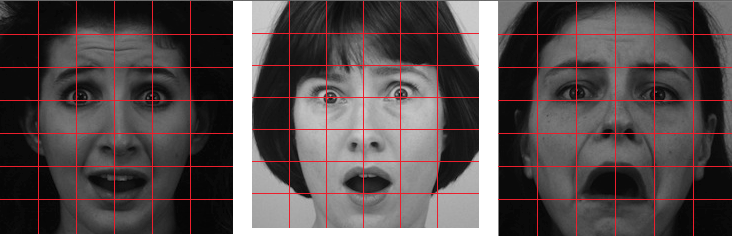
\includegraphics[scale=0.3]{figures/implementation_weight_example} 
\newline
\caption{Example of division into regions of face images from the KDEF database}
\label{implementation_weight_example}
\end{center} 
\end{figure}

\noindent GIVE RESULTS WITH WEIGHTS APPLIED
\newline

\noindent Another way to improve the LBP operator would be to use one with larger scale, hence modify the radius of the circular operator; for example, $ LBP_{12,2.5}^{u^2} $ or $ LBP_{16,4.0}^{u^2} $ (with $ P = 12 $ and $ R = 2.5 $ or with $ P = 16 $ and $ R = 4.0 $). This implies to use the bilinear interpolation because sampling points do not fall exactly on pixels, as seen in Chapter~\ref{chap:lbp}. However, using bilinear interpolation is more computationally expensive. A good compromise has to be found between computation time and accuracy rate.
\newline

\subsection{Combination of feature extraction methods}

\vspace{\baselineskip}
\noindent To improve the accuracy of LBP feature extraction method, another feature extraction method can be used and combined with it. 
\newline

\noindent  For example, a method has been proposed by Liao et al. \cite{LIA09}, where they combine LBP and Gabor filter. It is called Dominant Local Binary Patterns (DLBP), and is robust against change of lighting, image rotation and image noise.  It works by using the most recurrent patterns of the LBP method to obtain more information on the texture. It also uses the Gabor method to add global texture information to one already obtained by LBP. It works based on the circularly symmetric Gabor filter responses \cite{LIA09}. Figure~\ref{combination_lbp_gabor} contains two face images of the YaleB face database , and shows the robustness of the combination against change in lighting. Image (a) is the original image with different lighting conditions, and image (b) is the preprocessed image with the Gabor wavelets. Image (c) is the same image, mapped with the LBP operator. Finally, image (d) is the preprocessed image with the combination of the two methods \cite{GOH11}.
\newline

\begin{figure}[!h]
\begin{center}
\noindent 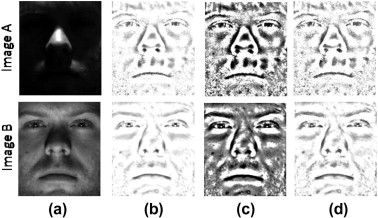
\includegraphics[scale=1]{figures/combination_lbp_gabor} 
\newline

\caption{2 face images of the YaleB face database (a) when processed with Gabor wavelets (b), LBP (c), and Gabor wavelets+LBP (d)\cite{GOH11}}
\label{combination_lbp_gabor}
\end{center} 
\end{figure}

\noindent  LBP has also been combined with the Scale Invariant Feature Transform descriptor (SIFT), which is a ROI descriptor. This descriptor is robust against image rotation, image translations, scaling and lighting variations. Heikkila et al. introduced a combination of the SIFT descriptor with the LBP operator \cite{HEI09}.
\newline

\bibliography{bib/mybib}
\label{bib:mybiblio}
\appendix
\chapter{Appendix A name}\label{ch:appAlabel}
Here is the first appendix

\end{document}
